%%%%%%%%%%%%%%%%%%%%%%%%%%%%%%%%%%%%%%%%%%%%%%%%%%%%%%%%%%%%%%%%%%%%
% Authors: A. Herrera-Poyatos, F. Herrera
% Tittle: Algoritmo memético equilibrado con diversificación voraz
% 							 CAEPIA 2015
%%%%%%%%%%%%%%%%%%%%%%%%%%%%%%%%%%%%%%%%%%%%%%%%%%%%%%%%%%%%%%%%%%%%

\section{Map Reduce}

	\subsection*{¿Qué es Map Reduce?}

		\begin{frame}{¿Por qué surge Map Reduce?}
			
				
			\begin{columns}
				\column{0.7\textwidth}
					\fontsize{10}{8}\selectfont	
					{\centering\color{TurkishRose}\textbf{Problemas de la programación distribuida}}
					\fontsize{9}{8}\selectfont	
					\begin{itemize}
						\item Implementaciones a bajo nivel: OpenMP, MPI ...
						\item Reimplementación de paralelismos equivalentes
						\item Implementación de la tolerancia a fallos
					\end{itemize}
					\kern3mm
					\fontsize{10}{8}\selectfont	
					{\centering\color{ChetwodeBlue}\textbf{Map Reduce}}
					\fontsize{9}{8}\selectfont	
					\begin{itemize}
						\MyPitem Nuevo paradigma de programación distribuida
						\MyPitem Simple, eficiente y de alto nivel
						\MyPitem Basado en las funciones map y reduce
						\MyPitem Gestiona los datos y la tolerancia a fallos
					\end{itemize}
				\column{0.3\textwidth}
				
					
\includegraphics[width=\textwidth]{./Images/google.png}
					
					\centering
					
\includegraphics[width=0.6\textwidth]{./Images/mapreduce-logo.png}
			\end{columns}		

			\kern3mm
			\begin{tcolorbox}[colback=ChetwodeBlue!10,colframe=ChetwodeBlue!60]
				\centering
				\fontsize{10}{8}\selectfont	
				\textbf{Ejemplo en un lenguaje funcional}
				\fontsize{9}{8}\selectfont								

				\kern 1mm	
				$f(x) = x^2$

				\kern 1mm
				$reduce(+, map(f, [1,2,3])) = reduce(+, [1,4,9]) = 14$
			\end{tcolorbox}	
		\end{frame}


		\begin{frame}{¿Cómo funciona map reduce?}
			
			\fontsize{7}{8}\selectfont	
			\centering
			
			\noindent\makebox[\linewidth]{\rule{\textwidth}{0.4pt}}			
			\textbf{Algoritmo:} Obtención del número de ocurrencias de cada una de las palabras de un texto.
			\noindent\makebox[\linewidth]{\rule{\textwidth}{0.4pt}}

			\kern2mm					
			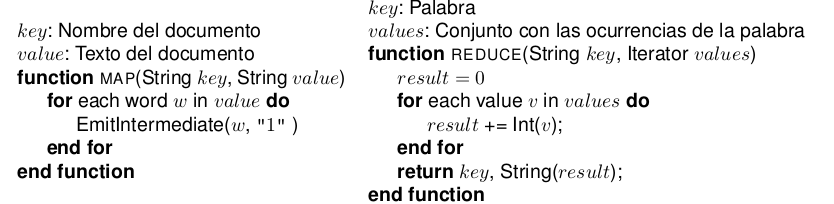
\includegraphics[width=0.88\textwidth]{./Images/count-words.png}		


			\noindent\makebox[\linewidth]{\rule{\textwidth}{0.4pt}}

			\kern2mm					
			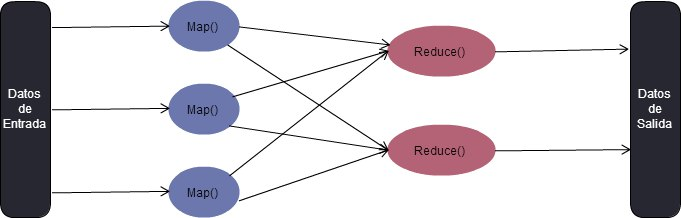
\includegraphics[width=0.9\textwidth]{./Images/MapReduce.jpg}
		\end{frame}


		\begin{frame}{¿Cómo funciona map reduce?}
			\fontsize{6}{8}\selectfont
			\centering
			\begin{tikzpicture}
			\node (img1) {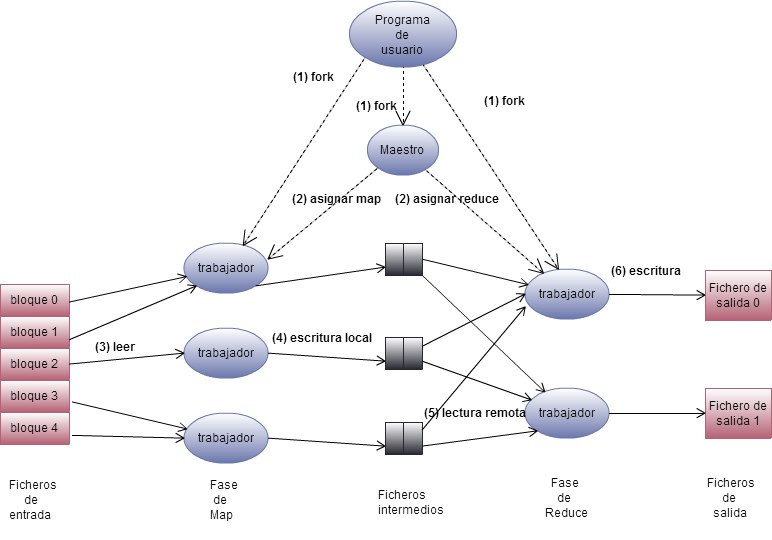
\includegraphics[width=0.9\textwidth]{./Images/MapReduce-MasterWorkers.jpg}};
			\node [above left = 2.5cm and 2cm of $(img1)$] (me) {\normalsize\textbf{Maestro - Esclavo}};
			\node [below = 3mm of $(me)$] (maestro) { \textbf{Maestro} $\twopartdef{{\color{TurkishRose}{\textbullet}}\  \text{Organiza los esclavos}}{{\color{TurkishRose}{\textbullet}}\ \text{Tolerancia a fallos}}$ };
			\node [below = 3mm of $(maestro)$] (esclavo) { \textbf{Esclavos} $\twopartdef{{\color{TurkishRose}{\textbullet}}\ Mapper \ (M)}{{\color{TurkishRose}{\textbullet}}\ Reducer  \ (R)}$ };
			\node [fill=TurkishRose!80,inner sep=2pt, text width=1.6cm, align=center, above right= 3cm and 3cm of $(img1)$] (pe) {Particionamiento de la entrada};
			\node [fill=ChetwodeBlue!80, inner sep=4.8pt, text width=1.4cm, align=center, below = 2.7mm of $(pe)$] (map) {Mappers};
			\node [fill=Jaguar!85, inner sep=2pt, text width=1.6cm, align=center, below = 2mm of $(map)$] (of) {\color{white}{Ordenación y filtrado}};
			\node [fill=ChetwodeBlue!80, inner sep=4.8pt, text width=1.4cm, align=center, below = 2.8mm of $(of)$] (re) {Reducers};
			\node [fill=TurkishRose!80,inner sep=2pt, text width=1.6cm, align=center, below = 2mm of $(re)$] (gs) {Generación de la salida};
			\path[draw=ChetwodeBlue!80,line width=2pt,->] ([xshift=3mm, yshift=3mm]pe.east) -- ([xshift=3mm, yshift=-3mm]gs.east);
			\end{tikzpicture}
		\end{frame}

	\subsection*{Software libre}
	
		\begin{frame}{}
			\kern-3mm
			\begin{center}
				
\includegraphics[width=0.7\textwidth]{./Images/hadoop.png}
				\kern-2mm
				\begin{tcolorbox}[colback=ChetwodeBlue!10,colframe=ChetwodeBlue!60]
					\fontsize{8}{8}\selectfont
					\centering
					\textbf{Open-source software for reliable, scalable, distributed computing}
				\end{tcolorbox}
			\end{center}
	
			\centering
			\kern-3mm
			\fontsize{6}{8}\selectfont
			\begin{itemize}
				\item HDFS: Sistema de archivos distribuido basado en Google File System (GFS).
				\item YARN: Gestión de tareas, recursos y nodos.
				\item SPARK: Map Reduce + procesamiento iterativo y en memoria.
			\end{itemize}

			\begin{tikzpicture}					
				\node (img1) {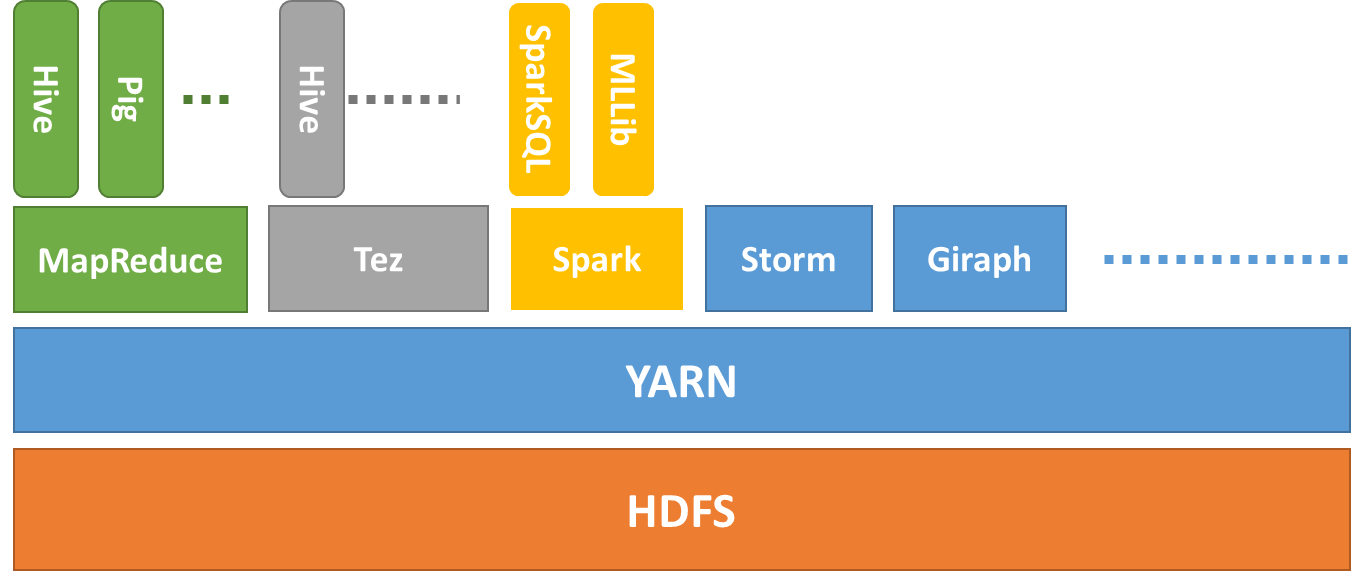
\includegraphics[width=0.8\textwidth]{./Images/hadoop-enviroment.png}};
				\node [above right = 0.5cm and 2cm of $(img1)$] (j) {
\includegraphics[width=0.2\textwidth]{./Images/java.jpg}};

			\end{tikzpicture}
						
		\end{frame}
